\chapter{Results}
\label{ch:results}

This chapter moves from component studies to the complete system.
The external comparison uses the full-SH protocol of \cref{ch:protocol}.

\section{Head-only adaptation}
\label{sec:exp:head}

Family heads are evaluated on assembled maps as well as on validation pairs.
The paired deployment study holds refinement active and disables thinning
in both arms. Improvements vary across scenes and families: ETH3D reports
$-29.1\%$ LPIPS, EuRoC $-20.8\%$, and four TUM sequences range from
$-7.9\%$ to $-25.9\%$. Replica adaptation is also beneficial in its
recorded study, whereas 7-Scenes is weak and ranges from a $0.14\%$ increase
to a $4.9\%$ decrease in LPIPS. These results do not imply that every
family or sequence benefits.

\begin{table}[t]
\centering\small
\begin{tabular}{@{}llrr@{}}
\toprule
Family & Sequence & $\Delta$PSNR (dB) & Relative $\Delta$LPIPS \\
\midrule
EuRoC & MH\_01 & $+0.62$ & $-20.8\%$ \\
TUM & desk & --- & $-7.9\%$ \\
TUM & room & --- & $-9.9\%$ \\
7-Scenes & chess & $+0.10$ & $+0.14\%$ \\
\bottomrule
\end{tabular}
\caption[Paired head-adaptation examples]{Family head versus released head,
with refinement enabled and thinning disabled in both arms. A dash denotes
a PSNR difference not tabulated here. Negative relative LPIPS is better.
These are separate adaptation runs, not the external-comparison maps.}
\label{tab:head}
\end{table}

A two-head, two-seed check gives relative differences below $5\%$ with
inconsistent signs at validation and deployment. Training uses an in-family
validation split.

\subsection{Tested explanations}
The variation in gains remains unexplained. \Cref{tab:falsified} records
four proposed explanations and the measurements that contradicted them.
The recorded $0.17\%$ LPIPS variation applies to those paired probes.

\begin{table}[t]
\centering\small
\setlength{\tabcolsep}{3pt}
\begin{tabular}{@{}p{0.30\linewidth}p{0.62\linewidth}@{}}
\toprule
Candidate & Why it fails \\
\midrule
Scale-frame consistency &
Mechanically inert: \cref{eq:splatt3rloss} is purely photometric, means are
\texttt{detach()}ed, and the metric-scale flag's only consumer is disabled.
Depth touches training solely via the mask. \\
Supervision coverage &
Measured per family: EuRoC has the \emph{lowest} coverage ($39.5\%$) and the
second-largest gain; ETH3D matches TUM's coverage ($61.9$ vs $60.0\%$) with
$3\times$ the gain. \\
Opacity un-saturation &
Explains four families in rank order but 7-Scenes measures $0.479$ ---
comparable to EuRoC's $0.38$ --- with a null gain. A measured counterexample,
not a pending cell. \\
Base-checkpoint headroom &
$\rho=0.145$ over $11$ sequences. ETH3D \texttt{sofa\_1} has the lowest
deficit of any sequence and the second-largest gain. \\
\bottomrule
\end{tabular}
\caption[Four falsified attributions]{Four pre-registered mechanisms for the cross-family variation, each
killed by measurement. The variation is real and remains unattributed.}
\label{tab:falsified}
\end{table}


\section{Injection-time thinning}
\label{sec:exp:thin}

Across twelve online comparisons spanning four datasets, six heads and
eight scenes, ten cells improve LPIPS clearly and two are near zero. The
worst measured change is a $0.16\%$ increase. Confidence-weighted versus
uniform allocation has a median difference of only $-0.06\%$, with its
interval spanning zero. The evidence supports opacity attenuation more
strongly than this particular allocation rule.

\begin{table}[t]
\centering\small
\begin{tabular}{@{}llr@{}}
\toprule
Scene & Head & Relative $\Delta$LPIPS \\
\midrule
Replica office3 & Plain adapted & $-12.7\%$\\
Replica office0 & Plain adapted & $-12.6\%$\\
Replica office2 & Plain adapted & $-10.2\%$\\
Replica room0 & Plain adapted & $-8.9\%$\\
Replica room1 & Plain adapted & $-7.1\%$\\
Replica office1 & Plain adapted & $-1.6\%$\\
Replica office0 & Opacity knee 0.9 & $-5.3\%$\\
Replica office0 & Opacity knee 0.6 & $-1.8\%$\\
TUM desk & Released & $-6.4\%$\\
TUM desk & Adapted & $-0.6\%$\\
EuRoC MH\_01 & Adapted & $-5.6\%$\\
7-Scenes chess & Adapted & $+0.16\%$\\
\bottomrule
\end{tabular}
\caption[Fine-grained opacity attenuation ablation]{Relative LPIPS change
for confidence-ranked attenuation with $\lambda=0.45$ versus off.
Refinement is active in both arms. Negative values improve LPIPS.}
\label{tab:thinning}
\end{table}


\subsection{Dose--response}
Two tested opacity regimes yield thinning gains of $-21.0\%$ and
$-15.8\%$ LPIPS. Without thinning, refinement itself changes median opacity
from approximately $1.0$ to $0.26$ in a released-head TUM map.
These findings show that insertion starts the map closer to an opacity state
that refinement can reach.

\section{Opacity and input luminance}
\label{sec:exp:mech}

\Cref{tab:lum} reports the registered sign test. The two Replica heads
trained with synthetic darkening have negative opacity--luminance
correlations; the three real-data heads have positive correlations.
All five tested heads match the predicted sign. The set contains two Replica
augmentation heads and three real-data heads. The SH residual and visibility
can also affect the correlation.

\begin{table}[t]
\centering\small
\begin{tabular}{@{}llr@{}}
\toprule
Head & Training data & $\rho(\alpha,\text{luminance})$ \\
\midrule
photospatial & Replica + synthetic darkening & $-0.316$ \\
mixed        & Replica + synthetic darkening & $-0.279$ \\
TUM          & real sensor                   & $+0.303$ \\
ETH3D        & real sensor                   & $+0.392$ \\
EuRoC        & real sensor                   & $+0.304$ \\
\bottomrule
\end{tabular}
\caption[Opacity--luminance correlations on five heads]{Registered
opposite-sign prediction, matched by five tested heads: two Replica
augmentation heads and three real-data heads. This correlation experiment
does not establish a unique causal interpretation of opacity.}
\label{tab:lum}
\end{table}


\section{Rendering: Replica, all eight scenes}
\label{sec:exp:replica}

\Cref{tab:replica} compares monocular maps from the released head with
fixed centres, thinning disabled and $300$\,s polish against Photo-SLAM.
Our mean is $23.019$\,dB versus $19.483$\,dB, a $3.536$\,dB difference.
PSNR is higher on all eight scenes. Mean LPIPS is $0.135$ versus $0.163$,
with improvements on five scenes; Photo-SLAM is better on office2,
office4 and room2. PSNR differences range from $0.23$\,dB on room1 to
$7.64$\,dB on room0. Replica optimisation budgets are not matched.

\begin{table}[t]
\centering\small
\setlength{\tabcolsep}{3.5pt}
\begin{tabular}{@{}lrrrr@{}}
\toprule
& \multicolumn{2}{c}{PSNR (dB) \up} & \multicolumn{2}{c}{LPIPS \dn}\\
Scene & Photo-SLAM & Ours & Photo-SLAM & Ours\\
\midrule
office0 & 22.19 & \textbf{26.30} & 0.219 & \textbf{0.104} \\
office1 & 17.77 & \textbf{22.08} & 0.190 & \textbf{0.115} \\
office2 & 20.15 & \textbf{20.97} & \textbf{0.135} & 0.150 \\
office3 & 19.20 & \textbf{20.18} & 0.165 & \textbf{0.144} \\
office4 & 16.43 & \textbf{23.65} & \textbf{0.129} & 0.156 \\
room0 & 17.81 & \textbf{25.44} & 0.159 & \textbf{0.110} \\
room1 & 21.68 & \textbf{21.91} & 0.181 & \textbf{0.139} \\
room2 & 20.64 & \textbf{23.62} & \textbf{0.123} & 0.160 \\
\midrule
Mean & 19.48 & \textbf{23.02} & 0.163 & \textbf{0.135} \\
\bottomrule
\end{tabular}

\caption[Rendering on Replica, all eight scenes]{Replica reconstruction
with monocular input and full exported SH. Bold identifies the better value
per scene and metric. Ours uses the released head, fixed centres, no thinning
and 300\,s polish. PSNR improves on eight scenes and LPIPS on five;
optimisation budgets and primitive counts differ.}
\label{tab:replica}
\end{table}


\begin{figure}[t]
  \centering
  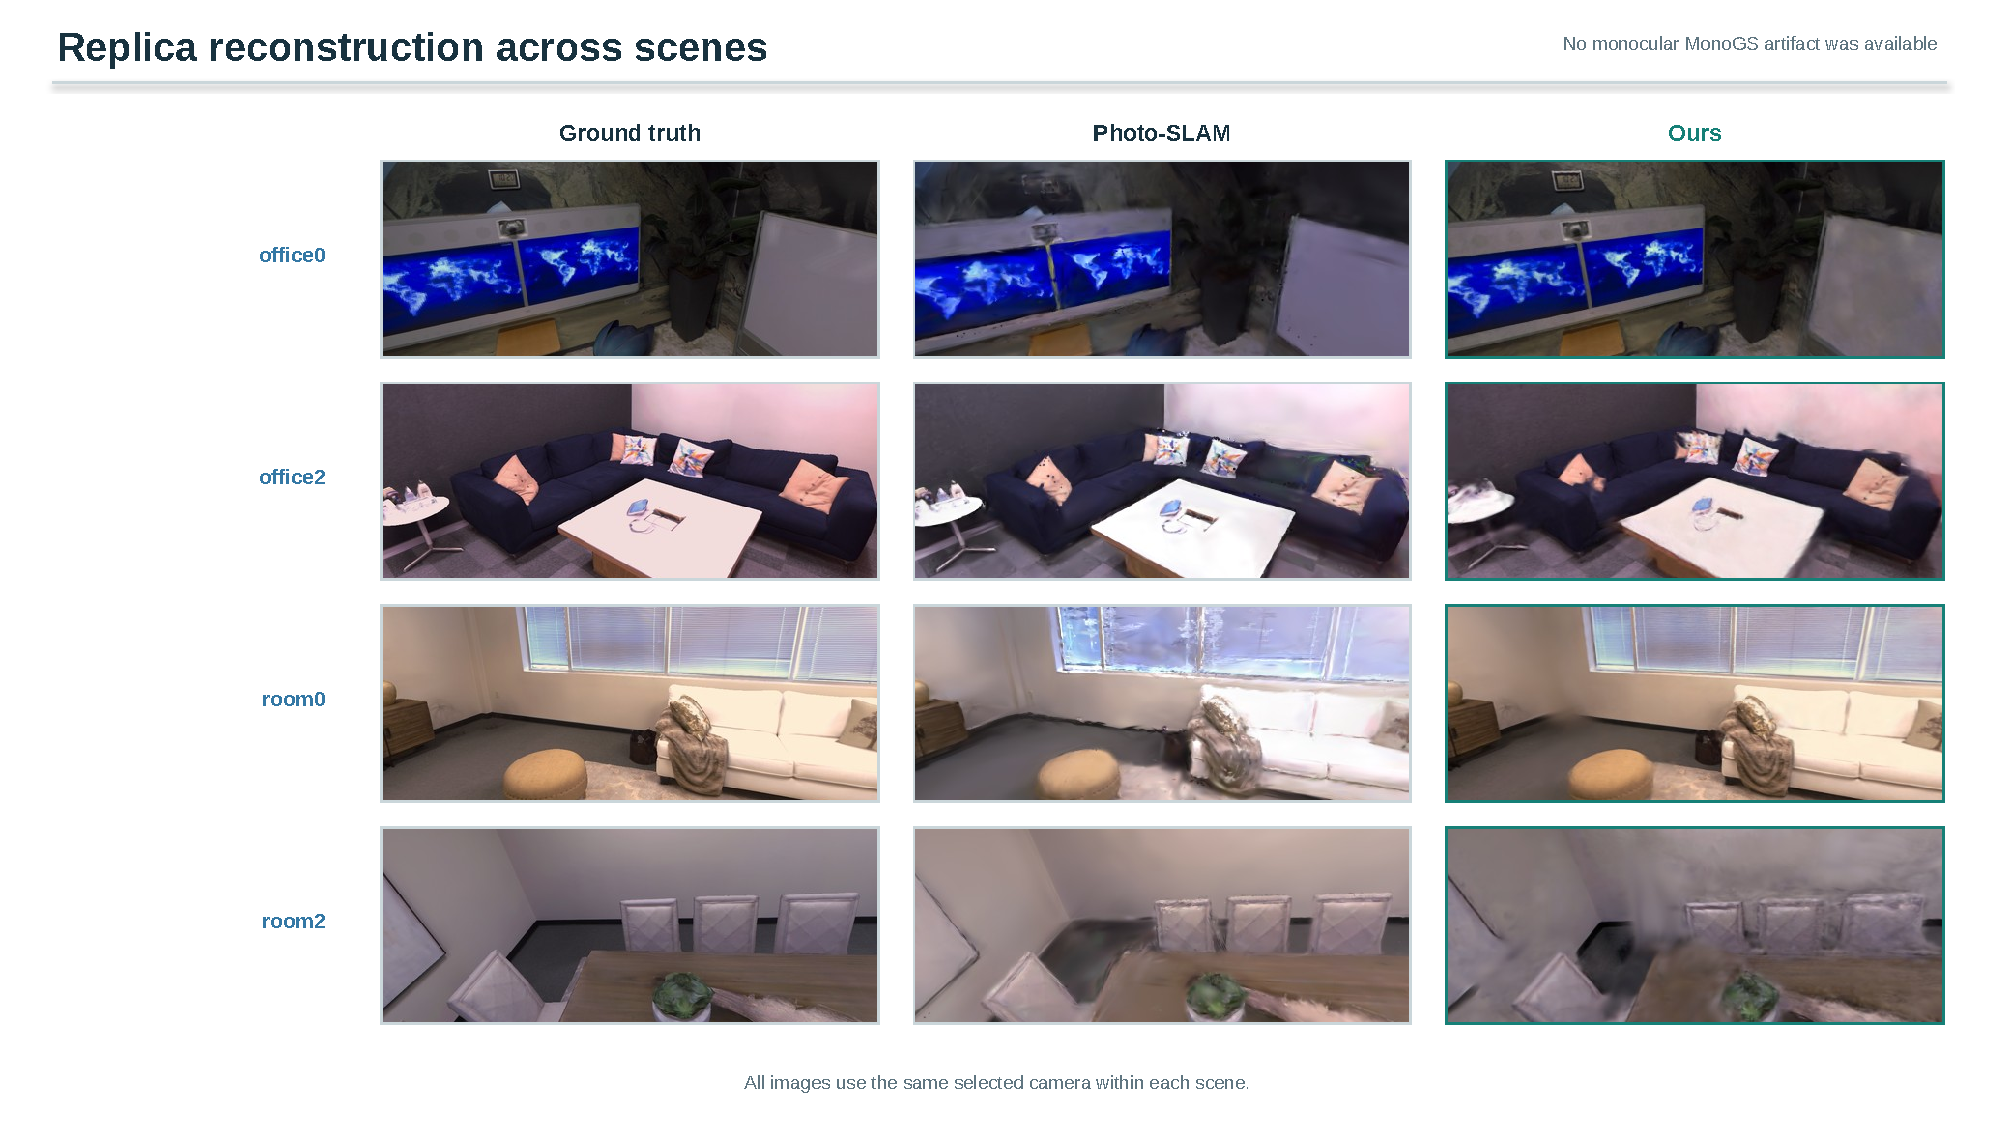
\includegraphics[width=\linewidth]{ral/fig/qualitative-replica.pdf}
  \caption[Replica qualitative comparison]{Ground truth, Photo-SLAM, and
  Splatt3R-SLAM on four Replica scenes. Each row uses one common evaluation
  camera. MonoGS is absent because no comparable monocular Replica map was
  available.}
  \label{fig:qualitative-replica}
\end{figure}

\begin{figure}[t]
  \centering
  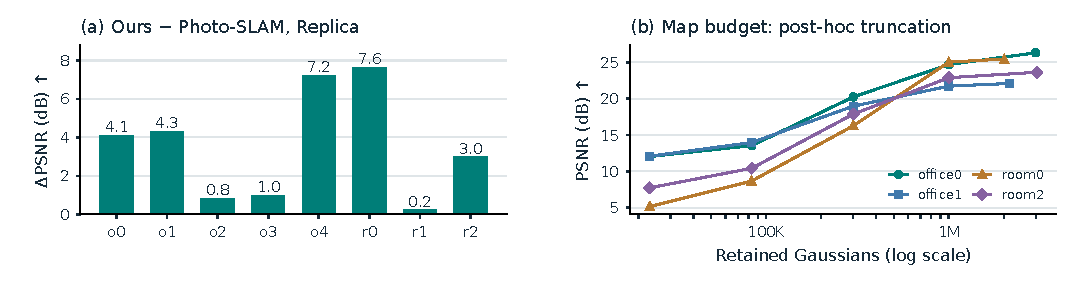
\includegraphics[width=\linewidth]{ral/fig/evidence.pdf}
  \caption[Scene dependence and map truncation]{(a) Fresh full-SH Replica
  scene PSNR differences; o/r denote office/room. (b) A separate recorded
  experiment retaining the highest-opacity primitives in four of our maps,
  without re-optimisation. Final markers denote full maps. The truncation
  curve measures sensitivity to this procedure, not optimal quality under
  each primitive budget.}
  \label{fig:evidence}
\end{figure}

\subsection{Scene aggregates and per-frame distributions}

A scene score aggregates MSE before taking the logarithm. It need not rank
methods like the median of per-frame PSNR differences.
\Cref{tab:frame-distribution} derives both statistics from the same $100$
frames used in each fresh comparison. On office2 and room1 the scene
difference is positive but the median frame difference is negative, and our
method wins only $42$ and $38$ frames, respectively.
On room0 the median difference is $+7.498$\,dB, but Photo-SLAM still has
the higher PSNR on $24$ frames.

\begin{table}[t]
  \centering\small
  \begin{tabular}{@{}lrrr@{}}
\toprule
Scene & Scene $\Delta$PSNR & Frame median & Positive frames\\
\midrule
office0 & +4.115 & +3.543 & 100/100 \\
office1 & +4.312 & +3.041 & 87/100 \\
office2 & +0.822 & -1.124 & 42/100 \\
office3 & +0.977 & +0.058 & 51/100 \\
office4 & +7.215 & +5.826 & 77/100 \\
room0 & +7.637 & +7.498 & 76/100 \\
room1 & +0.230 & -0.697 & 38/100 \\
room2 & +2.983 & +3.294 & 73/100 \\
TUM desk & +0.035 & -0.411 & 41/100 \\
\bottomrule
\end{tabular}

  \caption[Per-frame PSNR differences]{Ours minus Photo-SLAM on Replica,
  and Ours minus MonoGS on TUM desk. Scene $\Delta$PSNR uses each method's
  mean frame MSE; frame median uses paired per-frame PSNR differences.
  Positive frames counts strict numerical wins.}
  \label{tab:frame-distribution}
\end{table}

Representative images use the two middle ranks of these paired differences.
The office0 teaser and TUM qualitative figure therefore show typical
differences under a reproducible selection rule, rather than the largest
positive margins.

\section{Rendering: TUM desk and optimisation budget}
\label{sec:exp:tum}

\Cref{tab:tum} reports $13.949$\,dB for our map and $13.914$\,dB for
MonoGS. MonoGS has lower LPIPS,
$0.395$ versus $0.411$. Both exceed Photo-SLAM under this protocol.
Our $300$\,s polish and MonoGS's $339$\,s colour refinement are close in
duration, but total pipeline costs differ. This three-method rendering
comparison covers one TUM sequence.

\begin{table}[t]
\centering\small
\setlength{\tabcolsep}{4pt}
\begin{tabular}{@{}lrrr@{}}
\toprule
Method & PSNR (dB) \up & LPIPS \dn & $N$ (thousands)\\
\midrule
Photo-SLAM & 10.67 & 0.562 & 36.1 \\
MonoGS & 13.91 & 0.395 & 23.0 \\
Ours & 13.95 & 0.411 & 2396.9 \\
\bottomrule
\end{tabular}

\caption[Rendering on TUM \texttt{fr1\_desk}]{TUM desk reconstruction at
common cameras, retaining full exported SH. Ours uses 300\,s polish and
MonoGS 339\,s colour refinement; total pipeline compute is not matched.
$N$ counts exported primitives. This three-method rendering comparison
covers one sequence.}
\label{tab:tum}
\end{table}


\begin{figure}[t]
  \centering
  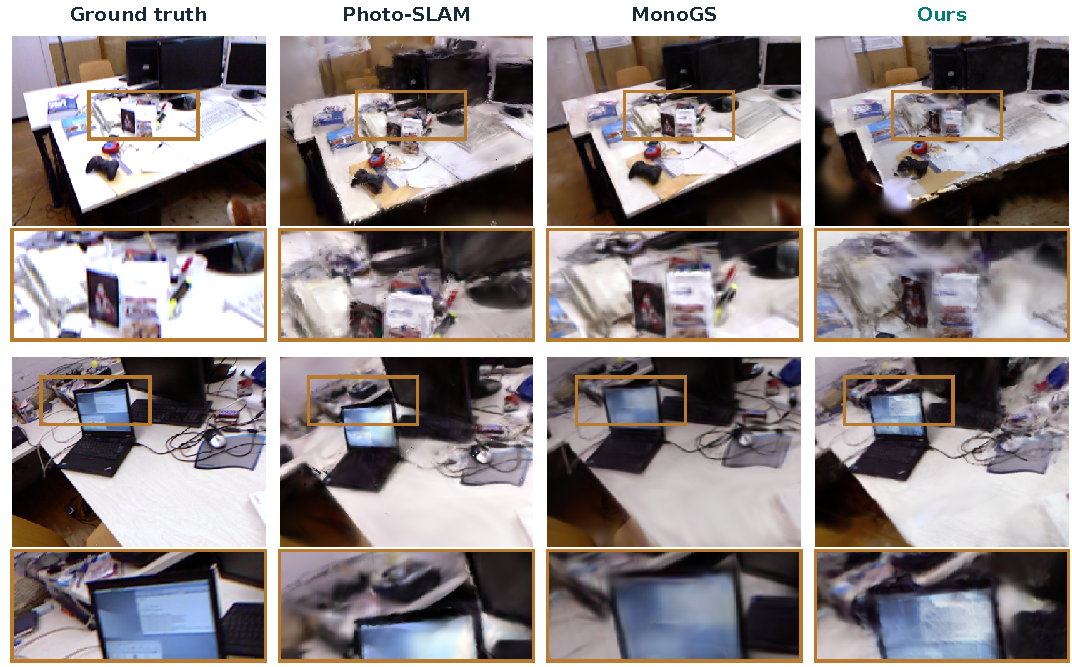
\includegraphics[width=\linewidth]{ral/fig/qualitative_tum.pdf}
  \caption[Four-column TUM reconstruction comparison]{Ground truth,
  Photo-SLAM, MonoGS and Ours, at two common TUM desk cameras. Each full
  view is followed by an identical crop, indicated in orange. Views occupy
  the two middle ranks of Ours-minus-MonoGS per-frame PSNR. Remaining blur
  and geometric distortion are visible in both MonoGS and our maps.
  No per-image score labels are used.}
  \label{fig:qualitative}
\end{figure}

Only $41$ of the $100$ TUM frames have higher PSNR for our method than
MonoGS, and the median difference is $-0.411$\,dB. This complements the
close scene aggregate and cautions against treating it as uniform visual
superiority. A separate historical $1200$\,s polish experiment reached
$14.61$\,dB and $0.379$ LPIPS under its original scoring configuration;
it measures additional-budget behaviour and is not a row in the fresh
common-budget comparison.

\section{Trajectory accuracy}
\label{sec:exp:ate}

\Cref{tab:ate} reports all nine TUM sequences. Our mean ATE is essentially
the same as MASt3R-SLAM's, consistent with preserving its geometric path.
This is a tracking-preservation control rather than a new tracking result.
Photo-SLAM is most accurate on several sequences but has large errors on
desk2, room and teddy. MonoGS also has large errors on several runs, which
strongly influence its mean. Multi-threaded tracking is not deterministic:
two Photo-SLAM desk runs yielded $0.0174$ and $0.0149$\,m ATE.

\begin{table}[t]
\centering\small
\setlength{\tabcolsep}{3pt}
\begin{tabular}{@{}lrrrrr@{}}
\toprule
Seq. & Ours & MASt3R & VGGT & Photo & MonoGS \\
\midrule
360   & 0.042 & 0.048 & 0.050 & \best{0.035} & 0.177 \\
desk  & 0.017 & 0.016 & 0.025 & \best{0.015} & 0.036 \\
desk2 & 0.028 & \best{0.024} & 0.029 & 0.438 & 0.844 \\
floor & 0.027 & 0.025 & 0.099 & \best{0.013} & 0.539 \\
plant & \best{0.015} & 0.020 & 0.025 & 0.046 & 0.071 \\
room  & \best{0.059} & 0.061 & 0.064 & 0.510 & 0.791 \\
rpy   & \best{0.022} & 0.023 & 0.026 & 0.057 & 0.041 \\
teddy & 0.048 & 0.045 & \best{0.036} & 0.305 & 0.123 \\
xyz   & \best{0.009} & \best{0.009} & 0.014 & 0.010 & 0.017 \\
\midrule
Mean  & \best{0.030} & \best{0.030} & 0.041 & 0.161 & 0.293 \\
\bottomrule
\end{tabular}
\caption[Trajectory accuracy, TUM freiburg1, five systems]{ATE RMSE (m), TUM freiburg1, all nine sequences and all five systems.
Photo-SLAM is non-deterministic (ORB-SLAM3 is multi-threaded): \texttt{desk}
gave $0.0174$ and $0.0149$ on two runs, so its single-run figures carry
run-to-run variance.}
\label{tab:ate}
\end{table}


\section{Shared anchors and refinement}
\label{sec:exp:refiner}

\subsection{Pose-correction control}
A blockwise $\mathrm{Sim}(3)$ test applies a 6\% scale correction to saved
TUM desk and room anchors. With fixed world-space supervision cameras,
refinement largely reverses the correction after about 500 steps. With
anchor-carried supervision, it is retained. This controlled test supports
the coordinate relation in \cref{eq:anchorconsistency}.

\subsection{Refinement on and off}
\Cref{tab:refiner} separates several recorded refinement interventions.
Holding the released head fixed and toggling refinement with $300$\,s
polish gives $+8.69$\,dB on ETH3D sofa\_1, $+4.62$\,dB on Replica
office0, $+3.52$\,dB on TUM desk and $+1.00$\,dB on EuRoC V1\_01.
Their relative LPIPS improvements are $58.3\%$, $56.8\%$, $27.3\%$
and $14.5\%$. These are not instantaneous online gains.

\begin{table}[t]
\centering\small
\setlength{\tabcolsep}{4pt}
\begin{tabular}{@{}lrl@{}}
\toprule
Ablation & $\Delta$PSNR & Note \\
\midrule
Refiner on, ETH3D   & $+8.69$ & 300\,s polish \\
Refiner on, Replica & $+4.62$ & \\
Refiner on, TUM     & $+3.52$ & \\
Refiner on, EuRoC   & $+1.00$ & \\
\midrule
Causal replay, 120 it. & $+1.21$ & TUM desk \\
Second GPU, unthrottled & $+2.15$ & tracker 101 to 103\,ms \\
\midrule
Uniform vs.\ recency & $+0.34$ & held-out mean \\
Voxel dedup, 10\,mm & $-0.53$ & $-27.6\%$ map size \\
\bottomrule
\end{tabular}
\caption[Refinement ablations]{Refinement ablations. ATE is unchanged in every row
($0.016975$ vs.\ a $0.0170$ baseline in the deterministic configuration): the
map is strictly downstream of tracking, and the pre-registered failure
condition ``ATE moves at all'' never fired. Earlier fixed-map probes favoured
freezing centres at approximately 300 and 3000 steps; the broader causal study
did not support making this a universal online default. The dedup row is a map-size
control that costs quality when it fires without a recovery budget, not a
quality feature.}
\label{tab:refiner}
\end{table}


\section{Online delivery across dataset families}
\label{sec:exp:online}

The deployed path is measured separately with family heads, causal SLAM,
the GUI enabled and refinement on a second GPU. \Cref{tab:online} reports
quality before polish. Seven of nine sequences improve LPIPS; TUM room and
360 worsen it by $11.1\%$ and $20.6\%$, despite small PSNR gains.
The refiner does not write pose corrections.

\begin{table}[t]
\centering\small
\setlength{\tabcolsep}{2.7pt}
\begin{tabular}{@{}llrrrr@{}}
\toprule
Family & Sequence & Bake P & Refine P & $\Delta$P & $\Delta$L \\
\midrule
TUM & desk & 12.42 & 13.75 & +1.33 & $-7.5\%$ \\
TUM & room & 11.15 & 11.45 & +0.30 & $+11.1\%$ \\
TUM & 360 & 12.00 & 12.14 & +0.14 & $+20.6\%$ \\
7-Scenes & chess & 13.44 & 13.79 & +0.35 & $-4.8\%$ \\
7-Scenes & office & 11.64 & 11.74 & +0.10 & $-1.6\%$ \\
7-Scenes & pumpkin & 14.15 & 14.91 & +0.77 & $-4.1\%$ \\
EuRoC & MH\_01 & 10.17 & 11.67 & +1.50 & $-4.1\%$ \\
EuRoC & V1\_01 & 12.06 & 12.69 & +0.63 & $-13.0\%$ \\
ETH3D & plant\_1 & 20.42 & 22.22 & +1.80 & $-7.4\%$ \\
\bottomrule
\end{tabular}
\caption[Online delivery, GUI on, dual GPU]{Actual GUI-on, dual-GPU online delivery. P is PSNR in dB and L is
LPIPS; $\Delta L$ is relative, so negative is better. Seven of nine cells
improve LPIPS. TUM room and 360 gain a little PSNR but lose perceptual quality
under the in-sequence budget, exposing supervision starvation on their large
maps rather than a universal refiner improvement. ETH3D \texttt{cables\_1} is
omitted because its $0.5$-m scene and $0.1165$-m ATE make held-out rendering
alignment-dominated. The reported online values are from the pre-polish
delivery pass; the longer polish diagnostic is separated below.}
\label{tab:online}
\end{table}


Across these runs, refinement adds approximately $7$--$10\%$ frame time
with the GUI open. The head-only arm uses $19.8$--$39.6$~GB on GPU~0;
refinement adds $1$--$1.5$~GB there and uses $2.8$--$14.0$~GB on GPU~1.
The largest observed combination is $41.1$~GB plus $14.0$~GB.
The focused desk latency result therefore does not imply negligible
overhead throughout the broader campaign.

\subsection{Budget and centre-update diagnostics}

\begin{table}[t]
\centering\small
\begin{tabular}{@{}lrrrr@{}}
\toprule
Iterations & 120 & 500 & 1000 & 3000\\
\midrule
Causal PSNR & 13.651 & 14.394 & 14.475 & 14.412\\
Post-hoc PSNR & 13.800 & 14.322 & 14.352 & 14.375\\
\bottomrule
\end{tabular}
\caption[Refinement iteration-budget control]{TUM desk PSNR in the recorded
causal and post-hoc replay. Both arms use the same map-evaluation protocol.}
\label{tab:budget}
\end{table}


The iteration control in \cref{tab:budget} shows that most of the TUM desk
gain appears by 500 steps. Additional causal iterations do not improve
monotonically. In the broader campaign, the deployed desk/360/room maps
received only $104/114/190$ refinement
steps; post-sequence polish supplied $1581/3821/1856$ steps and improved
PSNR by $+1.97/+2.30/+2.22$\,dB and LPIPS by $-22.0/-8.3/-15.9\%$.
An offline proxy suggested a position-learning-rate explanation for the
online degradation, but the causal loop did not reproduce it.
The offline centre-freezing and band-limit choices did not supply a
general online fix. Optimisation budget and coverage are the main measured
differences between the short causal and long polish phases.

\section{System cost}
\label{sec:exp:cost}

\Cref{tab:cost} compares recorded TUM desk costs with the same GPU memory
sampler. Our refiner-off run takes $70$\,s and peaks at $21{,}035$\,MiB;
Photo-SLAM takes $28$\,s and $1{,}286$\,MiB. These costs do not include
our $300$\,s polish.
Our exported desk map has $2.397$ million primitives, against $36{,}069$
for Photo-SLAM and $23{,}019$ for MonoGS.

\begin{table}[t]
\centering\small
\setlength{\tabcolsep}{5pt}
\begin{tabular}{@{}lrrl@{}}
\toprule
System & Wall clock \dn & Peak GPU (MiB) \dn & Note \\
\midrule
Ours        & \phantom{0}70\,s & 21{,}035 & $6.47$\,fps, refiner off \\
Photo-SLAM  & \best{\phantom{0}28\,s} & \best{\phantom{0}1{,}286} & fastest and leanest \\
MonoGS      & 555\,s & \phantom{0}2{,}389 & $404$\,s of it optimisation \\
VGGT-SLAM   & \phantom{0}24\,s & \phantom{0}9{,}436 & no renderable map \\
\bottomrule
\end{tabular}
\caption[System cost, all four systems]{End-to-end cost on TUM
\texttt{fr1\_desk} ($613$ frames), one GPU held exclusively for the
measurement, the same $1$\,Hz sampler for every system. VGGT-SLAM's time is
not comparable to the other three in what it buys: it produces poses and a
point cloud, not a renderable map. Our peak memory is $16\times$
Photo-SLAM's and $8.8\times$ MonoGS's, and Photo-SLAM is $2.5\times$ faster
end-to-end. Our row has refinement disabled and does not include the
post-sequence polish used in the external rendering comparison.}
\label{tab:cost}
\end{table}


The dense per-pixel representation is one source of this cost, alongside
model, optimiser and rendering storage. Naive opacity-ranked truncation
degrades reconstruction sharply (\cref{tab:curve}). It motivates
direct optimisation under a primitive budget. \Cref{app:tables} gives
per-family costs and extended truncation measurements.
